\section{Results and discussion}

\begin{figure}
	\centering
		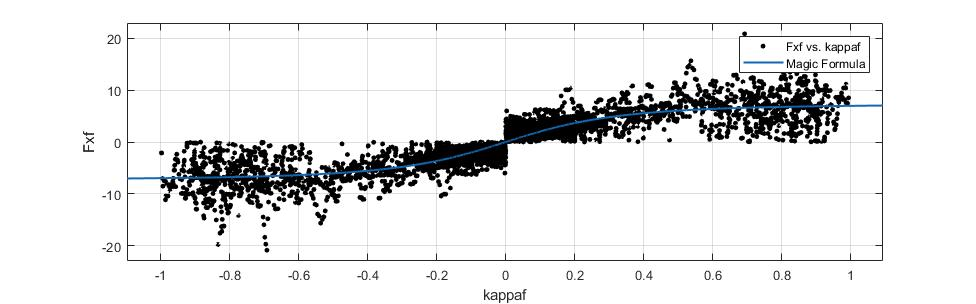
\includegraphics[scale=0.2]{figure/MagicFormulaFrontBags}
		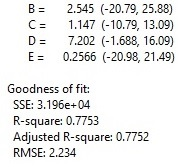
\includegraphics[scale=0.5]{figure/MagicFormulaFrontBagsFitnumbers}
		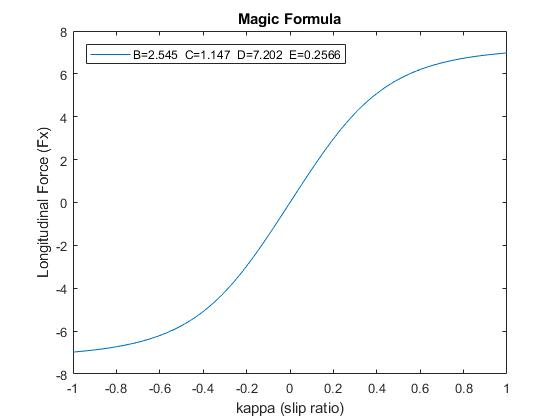
\includegraphics[scale=0.2]{figure/MagicFormulaFrontBagsPic}
		\label{fig:mffront}
\end{figure}
\begin{figure}
	\centering
		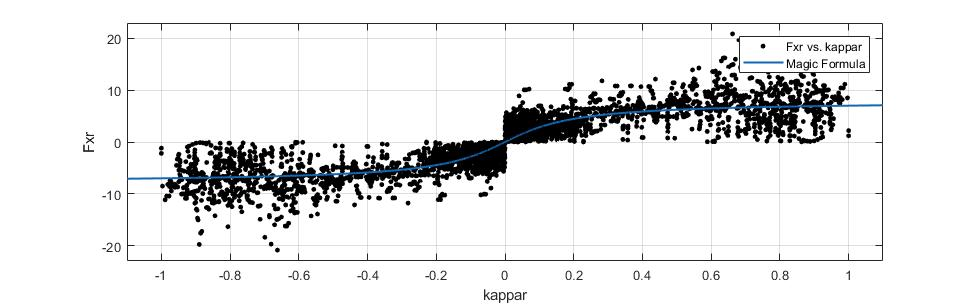
\includegraphics[scale=0.2]{figure/MagicFormulaRearBags}
		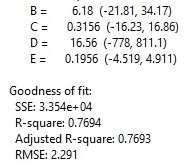
\includegraphics[scale=0.5]{figure/MagicFormulaRearBagsFitnumbers}
		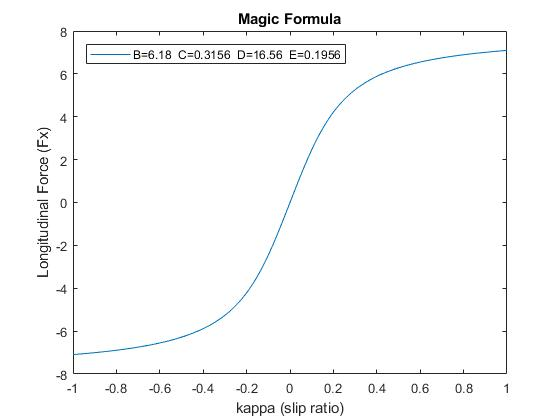
\includegraphics[scale=0.2]{figure/MagicFormulaRearBagsPic}
		\label{fig:mfrear}
\end{figure}
As noticeable from the pictures \ref{fig:mffront} and \ref{fig:mfrear}, the Magic Formula fits the points pretty descend. The accuracy of the fits is around R-square: 0.77. Furthermore, both the plots of the front and rear tires look similar. This had to be this case because we used the same tires for both front and rear. 
Even though the R-square of 0.77 is pretty good, there are still some minor errors in the plot. First of all, the Magic Formula has a peak and descend afterwards. This is not the case with our plots. It converges to a asymptote. Secondly, most magic formulas ascend much faster than our Magic Formula.
	There are a few possibilities why our Magic Formula differs from others. A possibility can be the data given by the revcounters. This data contains a lot of zeros because the sampling time of ROS is much faster than the sampling time of the Hall sensors. Because of this, interpolation between non-zero values is needed. This can result in inaccurate data. 

Another possibility is due to noise generated by our sensors:
Looking at figure [REFERENCE] we see a lot of noise generated in our plots compared to plots generated from other tests [misschien een Refererence]. There are two possible explanations to this noise. First is the RC car we used. As the aim at first was to improve the data acquisition software, not much was changed about the car itself. It wasn’t after much testing was done it became clear there were faults in the hardware design. One of the big problems discovered during testing was that having only two magnets per wheel generated a lot of zeros of distance traveled at our sampling rate of 120hz. This let to a need of a lot of signal filtering. Therefore wheels which were fitted with 24 magnets were created, however thusfore no testing with those have been done.

